% This is samplepaper.tex, a sample chapter demonstrating the
% LLNCS macro package for Springer Computer Science proceedings;
% Version 2.20 of 2017/10/04
%
\documentclass[runningheads]{llncs}
%
\usepackage{graphicx}
\usepackage{amsmath}
\usepackage[bookmarks]{hyperref}
\usepackage{color}
\usepackage{caption}
\usepackage{subcaption}
\usepackage{listings}
\usepackage{array}
\newcolumntype{L}[1]{>{\raggedright\arraybackslash}p{#1}}

\graphicspath{.}
% Used for displaying a sample figure. If possible, figure files should
% be included in EPS format.
%
% If you use the hyperref package, please uncomment the following line
% to display URLs in blue roman font according to Springer's eBook style:
% \renewcommand\UrlFont{\color{blue}\rmfamily}
\renewcommand{\floatpagefraction}{.8}%
\begin{document}
%\title{Credit Default Prediction with the American Express Dataset}
\title{Predicting Credit Card Default Using Deep Learning}
\titlerunning{Predicting Credit Card Default Using Deep Learning}

\author{Jonas Gann, Georg Grab}
%
% First names are abbreviated in the running head.
% If there are more than two authors, 'et al.' is used.
%
\institute{Rupert-Karls-University Heidelberg, Heidelberg, Germany\\
\email{\{jonas.gann, georg.grab\}@stud.uni-heidelberg.de}}
%
\maketitle              % typeset the header of the contribution
%
\begin{abstract}

% TODO TODO TODO TODO
Predicting credit card default is an important task for payment card providers to manage risk and take appropriate preventative action. It is often claimed that the tabular structure of performance indicators related to these events remains a unique challenge to deep learning based methods, despite their numerous breakthroughs in other domains. In this work, we aim to verify this claim by training and systematically analyzing several deep learning architectures for the task of credit default detection and subsequently comparing the results to a carefully tuned decision tree based classifier. The best performing deep learning architecture achieves a final evaluation score of $0.783$, whereas the decision tree based model achieves $0.791$. This result confirms prior work in the area of credit default prediction, stating that decision tree based models reach state-of-the-art performance that deep learning based method fail to surpass.

The code is publicly available at \url{https://github.com/J-Gann/AML}

\keywords{Credit Default Prediction  \and Gaussian Processes \and Deep Learning \and Time Series.}
\end{abstract}
%
%
%

% Deep Neural Networks and Tabular data: a survey https://arxiv.org/pdf/2110.01889.pdf

\section{Introduction}
\marginpar{Grab}

Credit cards have become an indispensable asset of everyday life, allowing quick and easy payments and borrowing. Owing to this simplicity, it is easy to forget that every time we swipe or touch the card, we enter into a legally binding agreement with the card provider to eventually pay back the money we owe. A default event in this context is defined as the failure of a debtor to do so over a predefined time period, for example, the passing of 180 days after issuance of the latest credit card statement. If such an event occurs, payment card providers typically assume that the debt will never be settled, close the account, and sell the account to a debt collection agency. As only a fraction of debt can typically be recovered by debt collection, the payment card provider incurs substantial losses if such events occur frequently \cite{beck2017determines}.
Assessing default risk is thus a vital part of business for lending institutions. Although there are centralized efforts to measure delinquency risk, such as credit scoring exist, payment card providers typically also develop in-house risk models. The Credit Default Prediction competition was organized by the payment card provider American Express in 2022 on the data science competition website Kaggle. Its purpose was to assess the performance of machine learning models when phrasing credit default prediction as a classification problem based on past performance indicators.

In this work, we investigate whether deep learning-based models can be successfully applied to this problem, where we define success as surpassing ensemble models in evaluation performance, as such models are typically the top performers in competitions based on similar tabular datasets \cite{shwartz2022tabular}. To do this, we participate in the Credit Default Prediction competition, developing several deep learning based models, and comparing their performance to a carefully tuned ensemble method based on gradient boosted decision trees.

Section \ref{sec:prereq} briefly introduces related work and the machine learning techniques utilized. Section \ref{sec:methods} elaborates in detail the challenge, the dataset on which it is based and the associated evaluation metrics, as well as our applied methodology, including preprocessing, training, and hyperparameter tuning. In Section \ref{sec:experiments} we present experimental results, which are discussed in Section \ref{sec:conclusion} along with associated limitations and possibilities for future work.



\section{Related Work}
\label{sec:prereq}
\marginpar{Grab}

This section gives a brief overview of previous work related to credit default prediction and associated machine learning methods.

% Talk about Credit default prediction in general
Due to the importance of assessing the default risk for various stakeholders, predictive models have been in demand for some time. Among the first risk models to find a major application is the Merton model proposed in 1974 \cite{merton1974pricing}, based on economic theory around company valuations and associated economic indicators. At the consumer level, the concept of credit scoring emerged as the primary measure of assessing default risk, where individual consumer actions are associated with a risk factor that accumulates in a global score per customer \cite{hand1997statistical}. Simple regression models remain a popular choice to calculate this metric in practice, as the deployment of black box approaches is often prevented from a regulatory perspective \cite{lee2021graph}. Among machine learning approaches for computing such risk scores, Support Vector Machines are being applied successfully \cite{trustorff2011credit} \cite{moula2017credit}, although Gradient Boosted Decision Trees (GBDT) and Nearest Neighbor approaches also show favorable results \cite{alam2020investigation}. In 2020, Alman et al. published a comprehensive investigation of machine learning techniques for the default prediction problem, comparing a wide variety of methods across several independent datasets. GBDT emerged as the best performing models \cite{alam2020investigation}, although deep learning based approaches were not included in this discussion. Such a comparative evaluation of GBDT and random forest based methods against deep learning approaches is provided in a 2018 report by Addo et al. \cite{addo2018credit}, the most similar prior work to ours we identified in the literature survey. In their analysis, logistic regression, GBDT, and random forest based models are compared with four different neural networks of varying complexity, the most complex of which has been selected through grid-based hyperparameter optimization. The results as measured by AUROC and the mean squared error on a dedicated testing dataset are in favor of GBDT and random forest models, with all neural network configurations failing to achieve higher test performance. However, Addo et al. only use simple neural network architectures consisting of fully connected layers, few hidden neurons, and a maximum depth of four, raising the question of whether more contemporary architectures would perform better.

The datasets used for credit default prediction are usually in the form of a tabular time series of past performance indicators. The application of machine learning methods to time series data has been studied extensively. Possible deep learning approaches include feed-forward and convolutional networks, as well as more specialized approaches such as long short-term memory and recurrent neural networks \cite{katarya2018study}. 

% Challenge that often comes up: dataset imbalance
A problem inherently associated with credit default prediction, which is often cited in the literature, is addressing dataset imbalance. As credit default is a rare event, the majority class of supervised training datasets are related to customers that do not default. Dataset imbalance in this context is usually addressed by undersampling the majority class or oversampling the minority class during training \cite{kubat1997addressing}. In the context of neural networks, weighted loss functions that result in steeper gradients for the minority class, such as focal loss, have been proposed \cite{lin2017focal}.

% Approaches for this type of data
% Talk about Trees vs DNN

\section{Materials and Methods}
\label{sec:methods}

In this section, we outline the materials and methods used to investigate the problem. First, we give a detailed overview of the challenge, the dataset on which it is based, and the evaluation metrics defined by the challenge organizers. Then, we describe the process of training and optimizing an ensemble model used for hyperparameter optimization as well as to provide a baseline performance measurement that can be compared to the deep learning based approaches described thereafter. Finally, we describe methods for evaluating and comparing our own models.

\subsection{The Dataset}
\label{sec:the-dataset}
\marginpar{Grab}

% Visualisierung: vielleicht eine Tabelle mit Anzahl der Features, pro Kategorie?
% TODO TODO TODO rede über dataset imbalance!!
The tabular dataset consists of a total of 5.5 million records, each consisting of 190 features. While a time point and the related customer ID are available for each record, the meaning of all other variables is partially obfuscated, with only the broad category in which the feature falls being revealed. The broad categories are delinquency, spend, payment, balance, and risk. Per customer, a maximum of 13 such records are available. According to the challenge description, these records represent an 18 months performance window after the latest credit card statement. Most variables are continuous, with only 11 of 190 features being categorical. Categorical features are represented by integers or strings. Missing values are frequent throughout the dataset, both with regards to single values and entire records. On average, 12.1 records are available per customer, and no single record in the training data exists with all values non-empty.

% TODO dieser Absatz sinnvoll?
% Eigentlich nicht, weil 0.57 auf training set berechnet. wieviel ist es auf test set? wäre interessant..
% The only feature whose meaning can be inferred from its usage in a document by the challenge organizers explaining the evaluation metric is the feature \emph{P\_2}. The document reveals that using the mean of the feature \emph{P\_2} as the default prediction achieves a score of $0.57$. This makes the interpretation likely that \emph{P\_2} is derived from an internal risk model at American Express, and thus reveals that the score of $0.57$ is an absolute minimum that a nontrivial machine learning model should be able to demonstrate.
% Note that last and first statement features seem the most important
% Notebook: 220827_catboost_feature_importance.ipynb


%\subsection{Importance of Features}
%\marginpar{Grab}
% TODO maybe a section "Data Exploration" somewhere.
% TODO or is it an experiment (Sec.4)?
To gain an initial overview of the available features despite anonymization, a preliminary exploratory analysis of the importance of the features was performed.
The importance of given feature categories can be quantified by training a decision tree-based ensemble model with minimal preprocessing and counting the frequencies of features that are used as split criteria. For this exploratory analysis, individual records were joined with the target variable and temporal information was removed. The model was trained using an ensemble of decision trees with gradient boosting. A validation split of $15\%$ was used to detect overfitting and perform early stopping. After training, feature importances were calculated using independent tree SHaP values \cite{lundberg2020local}. Fig. \ref{fig:feature_importances} shows the mean of feature importances calculated per feature category, with feature \emph{P\_2} plotted separately. The plot shows that the feature \emph{P\_2} is an outlier in terms of predictive performance in the resulting ensemble model, indicating that this feature already represents a type of default risk. For the remaining features, delinquency is on average the category with the highest explanatory power, followed by, in descending order, balance, payment, spend, and risk-related variables.

\begin{figure}
    \centering
    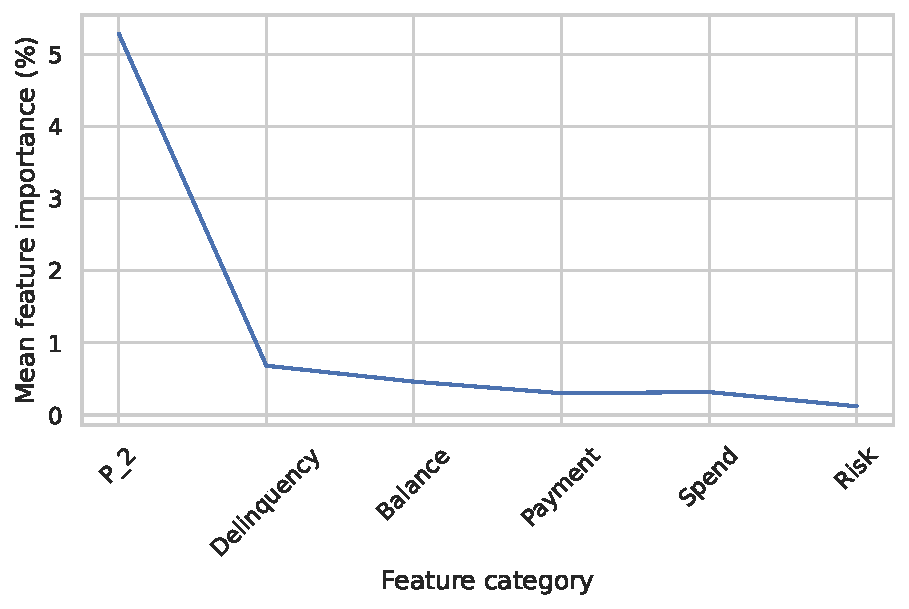
\includegraphics[width=0.8\textwidth]{220924_feature_importance_catboost_rowwise.pdf}
    \caption{Mean Feature Importance per Category using independent SHaP values \cite{lundberg2020local}, with outlier \emph{P\_2} shown separately.}
    \label{fig:feature_importances}
\end{figure}


\subsection{Design of the Challenge}
\label{sec:design-of-the-challenge}
\marginpar{Grab}

The challenge was held as a public event on the data science competition website Kaggle over a three month time window from May 2022 until August 2022. During that time, participants were free to register for the challenge, form teams, and submit candidate solutions derived from the competition dataset. Candidate solutions were submitted in the form of predictions of default probabilities on the challenge's publicly available testing dataset. Upon submission of such a candidate solution, the challenge evaluation metric would be computed for the entire test dataset, but only reported on a subset thereof making up approximately 51\% of all available data. This subset was kept secret by the challenge organizers. The evaluation metric achieved, called the public score, would be immediately published on a leaderboard that was public for the duration of the challenge. Only after passing of the challenge deadline, the evaluation metric achieved on the remaining 49\% would be revealed, referred to as the private score. This private score was then used for the final ranking of the participants.

\subsection{Official Evaluation Metrics}
\label{sec:evaluation-metrics}
\marginpar{Grab}

The mean of two separate ranking measures was used as the official evaluation metric of the challenge,

\begin{equation*}
    M = \dfrac{G+D}{2},
\end{equation*}

with $G$ the Normalized Gini Coefficient, and $D$ the default rate captured at $4\%$. The Normalized Gini Coefficient is a metric capable of describing the overall performance of a classifier across all possible operating points in a way equivalent to the more familiar Area under the Receiver Operating Characteristic curve (AUROC) \cite{schechtman2019relationship}. For the default rate at $4\%$, the predicted default probabilities are sorted in descending order. The metric is defined by calculating the true positive rate for the first $4\%$ of the predictions in this ordered list.

\subsection{Baseline Hyperparameter Tuning}
\marginpar{Grab}
\label{sec:baseline-hyperparam-tuning}

Data preprocessing poses a unique challenge for the given dataset for various reasons. First, the features are completely anonymized apart from a broad feature category, making preprocessing through manual feature engineering difficult. Second, missing values are frequent throughout the dataset, and lastly, the data is structured as a time series, with a variable amount of records available per customer. Therefore, multiple data preprocessing strategies have to be applied, each with associated hyperparameters.

% TODO more dataset related tuning
To systematically determine the appropriate preprocessing hyperparameters for the given dataset, a hyperparameter optimization strategy was devised. First, suitable hyperparameters are identified, and associated preprocessing routines are implemented using these parameters.  Then, using the data preprocessed according to a given set of hyperparameters, a baseline classifier is trained. Finally, this classifier is evaluated on a validation split according to the evaluation metrics defined in Section \ref{sec:evaluation-metrics}. This entire process is modeled as a function $f(x, \theta)$ with $x$ the raw input data and $\theta$ the set of hyperparameters, returning the final challenge evaluation metric. 

Using $x$ as a constant subset of the full input data for efficiency reasons and allowing $\theta$ to vary, an optimization problem can be formulated:

\begin{equation}
    \hat{\theta} = \arg\max_{\theta} f(x, \theta).
\end{equation}

While computing $\hat{\theta}$ exactly is intractable due to the large input space of potential hyperparameters and the fact that many local optima exist, good approximations can be obtained through Gaussian Process based hyperparameter optimization. To perform the optimization, the Optuna framework \cite{akiba2019optuna} was used.

Hyperparameters that are part of the optimization are listed in Table \ref{tab:hyperparam-opt}. Hyperparameters are part of the whole machine learning pipeline and, as such, both parameters related to dataset preprocessing, as well as parameters directly related to the predictor, are subject to optimization.

\begin{table}[h]
    \vspace{0.1cm}
    \centering
    \setlength{\tabcolsep}{0.5em}
    \def\arraystretch{1.1}
    \begin{tabular}{L{2.8cm} | L{4cm} | L{1.7cm} | L{2.5cm} }
    \hline
    \textbf{Hyperparameter} & \textbf{Description} & \textbf{Type} & \textbf{Range}\\
    \hline
    Impute Strategy \textsuperscript{($*$)}\ & Statistic used to impute missing values & Discrete & mean, median, most frequent\\
    Grouped Impute \textsuperscript{($*$)} & Impute based on global or per-customer statistics & Boolean & \emph{T}, \emph{F}\\
    Drop Percentage \textsuperscript{($*$)} & Delete columns with high correlation coefficient & Continuous & $[0.8; 0.99]$\\
    Denoise\textsuperscript{($*$)} & Apply denoising strategies & Boolean & \emph{T}, \emph{F}\\
    Depth & Tree depth & Integer & $\{3; 11\}$\\
    Iterations & Maximum number of trees to add to GBDT ensemble & Integer & $\{20; 150\}$\\
    Learning Rate & Learning rate for GBDT ensemble & Continuous & $[10^{-5}; 10^{-3}]$\\
    \hline
   \end{tabular}
   \vspace{0.1cm}
   \caption{Hyperparameters optimized for baseline regressor. Dataset related parameters ($*$) were reused for deep learning based experiments.}
   \label{tab:hyperparam-opt}
\end{table}

The first two dataset preprocessing parameters are related to imputation strategies.
Proper handling of such values plays an important role in the challenge dataset, as missing values are so frequent that simple strategies such as deleting incomplete customer records would result in deletion of the entire training data.

While more elaborate imputation techniques using machine learning based regressors exist, this analysis is restricted to simple strategies that fill missing values given a column statistic, as otherwise hyperparameter optimization proves intractable given the large volume of data. The optimization is subject to both the kind of statistic used for imputation - mean, median, or most frequent - as well as the conceptual level within which the imputation is performed. The latter is modeled as the boolean hyperparameter \emph{Grouped Impute} which, if true, performs imputation on the level of the customer time series and imputes based on global column statistics otherwise. Regardless of the \emph{Grouped Impute} setting, imputation based on the global column statistic is always carried out again at the end of preprocessing. The reason is that many instances of customer time series exist that do not have any value in a given column, and as such computing the column statistic fails if done on the time series level.

% TODO can we cite that high statistical correlation leads to worse model performance?
A further challenge associated with the dataset is that many features show a high degree of statistical correlation. Highly correlated features, in general, do not improve predictive performance and are known to decrease performance in some cases \cite{yoo2014study}. Using correlation coefficients, such features can be detected; however, it is not clear in general which threshold to use beyond which on selecting the threshold at which one of the highly correlated features should be deleted. Because of this, a \emph{Drop Percentage}  hyperparameter was added to the optimization, with possible values in the interval $[0.8; 0.99]$ tested.
%todo aboveabove...

Finally, analyzing the distributions of individual features reveals that uniform random noise in the range $[0, 0.01]$ might have been injected into the dataset. This claim stems from the fact that features with the majority of values distributed in the range $[0, 1]$ have minimum and maximum values that are slightly negative and slightly above one, respectively, with a maximum deviation of $0.01$. As most of the features are likely to describe money, which is a discrete quantity with increments of $\$0.01$, it is unlikely such values are naturally occurring in the dataset. A possible denoising strategy is to round the values to the nearest two significant digits. This is enabled in the preprocessing pipeline if the \emph{Denoise} parameter is enabled.

After all preprocessing steps outlined above are executed, the data is reshaped such that all records pertaining to one customer represent one row of the training data, with time series data added as additional columns.


The remaining hyperparameters in Table \ref{tab:hyperparam-opt} are related to the baseline classifier, a Gradient Boosted Decision Tree ensemble that is trained using a set of dataset hyperparameters, and evaluated to quantify their effect. 

\subsection{Gradient Boosted Decision Trees}
\label{sec:gbdt}
\marginpar{Grab}

This work uses Gradient Boosted Decision Trees (GBDT) in two ways. First, as described in the previous Section, a round of dataset hyperparameter optimization is concluded with training GBDT on the preprocessed data in order to obtain a value of $f(x, \theta)$. Second, the results of GBDT are used as a baseline for comparison against deep learning approaches, as GBDT is a strong method for tabular data in general and credit default prediction in particular \cite{addo2018credit}.
%Random Forest based ensemble approaches tend to perform well on tabular data.  In this work, they will be used to establish a performance baseline that the deep learning based approaches need to surpass in order to be useful.
%Bla Bla Catboost
The main idea of GBDT is to first take a naive guess, typically the mean, to predict the output variable, to calculate the residual between the guess and the actual value, and then incrementally refine this guess by sequentially chaining decision trees \cite{prokhorenkova2018catboost}. Every decision tree is designed to contribute a certain amount, quantified by a learning rate parameter, to refining the error of the previous decision tree in the chain, quantified by a differentiable loss function. Trees are added either until a predefined maximum tree count is reached, overfitting is detected as measured on a validation split, or the gradient of the loss function drops below a certain threshold.

In this work, we use the CatBoost implementation of GBDT, which additionally extends the gradient boosting algorithm in certain ways to make it work well on categorical features and noisy input data \cite{prokhorenkova2018catboost}. Data is preprocessed according to the strategy laid out in Section \ref{sec:baseline-hyperparam-tuning}. For the final predictions, GBDT related optimized  hyperparameters as summarized in Table \ref{tab:hyperparam-opt} are reused. Weighted binary cross entropy is used as the loss function in order to counteract dataset imbalance. The rest of the hyperparameters of the CatBoost classifier remain at their default values. The final predictions are computed by an ensemble obtained through 5-fold cross validation, with individual predictions averaged.


\subsection{Multi Layer Perceptron}
\marginpar{Gann}
\label{subsec:mlp}

As an initial approach to solving the classification problem with deep learning models, we utilize a Multi Layer Perceptron (MLP). A MLP is a feedforward artificial neural network consisting of multiple fully connected layers of perceptrons with a nonlinearity in between. An example of a single layer is shown in Figure \ref{fig:layer_mlp}. Here, one can see that an activation (which is the resulting numerical vector from the previous layer) is multiplied with a weight matrix in what is called a linear layer. The resulting output (which dimension is determined by the size of the activation and the weight matrix) is referred to as pre-activation to which an activation function is applied to generate the input used for the next layer.

\begin{figure}[h]
    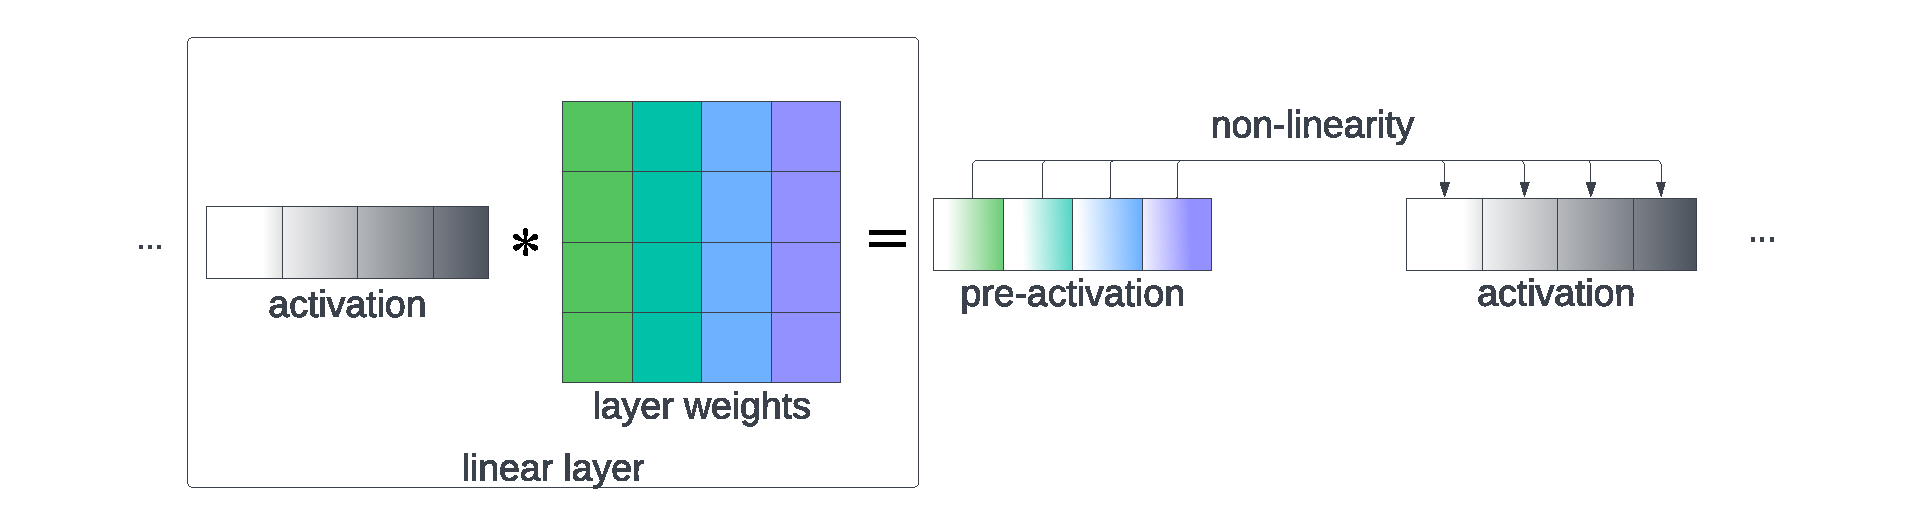
\includegraphics[width=\textwidth]{images/layer_mlp.pdf}
    \caption{MLP layer with associated terminologies.}
    \label{fig:layer_mlp}
\end{figure}

The first layer is commonly used to represent the input data in the form of a one-dimensional vector. The activation resulting from the last layer can be used as an output of the model. In the case of binary classification, the activation of the last layer usually is a Sigmoid function to map the pre-activation to a probability between 0 and 1.
As can be seen in Figure \ref{fig:layer_mlp} the input to a linear layer must be a one-dimensional numerical vector. Therefore, we can use the preprocessed dataset described in \ref{sec:baseline-hyperparam-tuning} which has, numerical and categorical variables combined, the shape $[367130, 2314]$ where 367130 is the number of entries in the dataset and 2314 is the feature size. Thus, each feature is the ordered concatenation of the 13 time series values of size 178 per customer.

The concrete architecture of the MLP was optimized using Optuna as will be shown in Section \ref{subsec:hyperparameter-tuning-fcn-cnn}.


\subsection{Convolutional Neural Network}
\marginpar{Gann}

\label{subsec:cnn}

The MLP described in the previous section is not a time-invariant approach to time series classification \cite{DBLP:journals/corr/abs-1809-04356}. This means that small local changes in the order of features can have a large effect on the overall classification. The reason is that each feature in an MLP has its own weight and cannot be shifted to the left or right. 
This behavior might be advantageous when each feature is independent of its neighboring features. However, for time series, this is typically not the case, as one can imagine patterns emerging at different time points and, therefore, different feature indices.
It might be of advantage to utilize a time-invariant approach, which could improve classification accuracy by enabling the model to better maintain a notion of order while learning features where local changes in the input can be limited to only have an effect on neighboring features during classification. This means that some characteristic time series could be detected at time point $t$ just as at time point $t+5$, thus making its detection invariant to its point in time.
One example of a time-invariant approach is the use of Convolutional Neural Networks (CNN), which in this case can use one-dimensional convolutions to learn filters for expressive feature generation.

We use the preprocessed dataset described in \ref{sec:baseline-hyperparam-tuning} for CNN training. However, the data needs to be modified to be usable as input data to the CNN. Therefore, we reshape the feature vector to $[178, 13]$, where 178 is the number of channels and 13 is the length of the time series. 
As shown in Figure \ref{fig:cnn_kernel} during the convolution, a one-dimensional kernel (marked red) of variable size (size 3 in this case) slides over the time series and applies its filter to the input values at each step. Using the "same" padding, the feature vector produced by the convolution can be expanded to retain its original size by replicating the first and last elements.

\begin{figure}[h]
    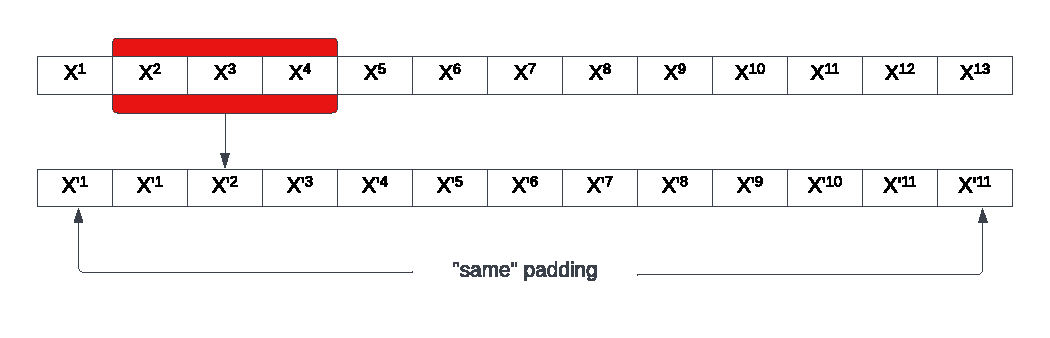
\includegraphics[width=\textwidth]{images/cnn_kernel.pdf}
    \caption{ One dimensional convolution over a time series of length 13 stride one, kernel size 3, and "same" padding.}
    \label{fig:cnn_kernel}
\end{figure}

This convolution process is performed for each of the input channels of a customer using individual kernels. The result of the convolution of each channel is summed up, resulting in a vector of size $[178, 1]$ when the "same" padding is used. To create multiple output channels, multiple convolutions can be performed and their results concatenated. In this way, multiple convolutional layers can be stacked, each with the same input and output shapes. 
The purpose of the CNN is to generate expressive features by learning various filters for each time series. A filter applied to a time series representing the credit balance could, for example, be learned to detect a sudden large reduction within an otherwise even value. This could be one of many indicators of default risk.

Each of the learned filters is time invariant, as they detect patterns independent of where they appear in the time series by being applied in a sliding operation as shown in Figure \ref{fig:cnn_kernel}. Therefore, a CNN approach for feature extraction of time series data takes advantage of the inherent structure of the time series, which can increase classification performance.


The features learned by the CNN are forwarded to an MLP that reduces the dimensionality to 1 for the final probability prediction of a credit default using a Sigmoid activation function.


The concrete architecture of the CNN is optimized using Optuna as discussed in Section \ref{subsec:hyperparameter-tuning-fcn-cnn}.





\subsection{MLP and CNN Training}
\marginpar{Gann}
\label{subsec:train-fcn-cnn}
Training was identical for both MLP and CNN despite differences in training hyperparameters described in Section \ref{subsec:hyperparameter-tuning-fcn-cnn}.

The data set was used as described in Section \ref{sec:baseline-hyperparam-tuning} as well as the adoptions described in Section \ref{subsec:mlp} and Section \ref{subsec:cnn}. We divided the data set into a training set and a validation set while 70\% of the data points remained in the training set.

We used binary cross-entropy as a loss function and trained for 9 epochs where each epoch consisted of the entire training set. In the training loop we logged the average loss of the batch, and after every 100 batches we evaluated the model against the validation set and logged the resulting average loss. After each epoch, we stored the current model to select the best performing model afterwards and multiplied the learning rate with an optimized learning rate decay factor. 




\subsection{MLP and CNN Hyperparameter Tuning}
\marginpar{Gann}

\label{subsec:hyperparameter-tuning-fcn-cnn}

We again use Optuna to optimize the hyperparameters of the MLP and CNN. The reason we again use automated hyperparameter optimization is that manually specifying hyperparameters such as number of layers, kernel size, output size, learning rate, and optimizer can take a very long time, and it is likely that without much experience, one does not find optimal values. However, the selection of hyperparameters to be tuned as well as the range in which they are optimized is still manual, giving the possibility of speeding up computation but leaving possibilities for missed optima.

For optimization, we used the adapted training data for the respective models as described in Section \ref{subsec:mlp} and Section \ref{subsec:cnn}. However, in order to get reasonable performance, we limited the size of the dataset to 10000 entries. To evaluate the performance of trials, we used the binary cross-entropy loss.

The hyperparameters selected for optimization are shown in Tables \ref{tab:hyperparam-opt-mlp} and \ref{tab:hyperparam-opt-cnn}.

\begin{table}[h]
    \vspace{0.1cm}
    \centering
    \setlength{\tabcolsep}{0.5em}
    \def\arraystretch{1.1}
    \begin{tabular}{L{4cm} | L{1.7cm} | L{2.5cm} }
    \hline
    \textbf{Hyperparameter}  & \textbf{Type} & \textbf{Range} \\
    \hline
    Number Linear Layers & Integer & 1 - 10 \\
    Size Linear layer k & Integer & 100 - 300 \\
    Activation & Discrete & LeakyReLU, ReLU, ELU \\
    Learning Rate & Continuous & 1e-7 - 0.1 \\
    Optimizer & Discrete & AdamW, Adam, SGD, Adagrad, NAdam \\
    Learning Rate Decay & Continuous & 0.4 - 0.99 \\
    Batch Size & Integer & 16 - 128 \\
    \hline
   \end{tabular}
   \vspace{0.1cm}
   \caption{Hyperparameters optimized for Multi Layer Perceptron}
   \label{tab:hyperparam-opt-mlp}
\end{table}


\begin{table}[h]
    \vspace{0.1cm}
    \centering
    \setlength{\tabcolsep}{0.5em}
    \def\arraystretch{1.1}
    \begin{tabular}{L{4cm} | L{1.7cm} | L{2.5cm} }
    \hline
    \textbf{Hyperparameter}  & \textbf{Type} & \textbf{Range} \\
    \hline
    Number Convolutional Layers & Integer & 1 - 30 \\
    Kernel Size Convolutional Layer k & Integer & 1 - 12 \\
    Out Channel Size Convolutional Layer k & Integer & 100 - 300 \\
    Convolution Activations & Discrete & LeakyReLU, ReLU, ELU \\
    Number Linear Layers & Integer & 1 - 10 \\
    Layer Size Linear Layer k & Integer & 100 - 300 \\
    Linear Activations & Discrete & LeakyReLU, ReLU, ELU \\
    Pooling after Convolution & Discrete & True, False \\
    Learning Rate & Continuous & 1e-7 - 0.1 \\
    Learning Rate Decay & Continuous & 0.4 - 0.99 \\
    Batch Size & Integer & 16 - 128 \\
    \hline
   \end{tabular}
   \vspace{0.1cm}
   \caption{Hyperparameters optimized for Convolutional Neural Network}
   \label{tab:hyperparam-opt-cnn}
\end{table}


The hyperparameters that were optimized concern either the model architecture or the training process. In the case of the MLP, the hyperparameters concerning the model architecture were the number of layers and the size of each layer. The trade-off here is between sufficient model complexity and overfitting as well as performance. 
Although ReLU activations are commonly used, we included some alternative activation functions in the optimization which might increase performance in some cases.

In case of the CNN, the hyperparameters concerning the model architecture were similar to the MLP, the number of layers, and output size, in this case for the linear layers as well as for the convolutional layers. In addition, we optimized the kernel size for each convolutional layer. As can be seen in Figure \ref{fig:cnn_kernel}, the size of the kernel has an effect on the size of the patterns that can be detected. It is not trivial to determine the suitable kernel sizes beforehand. In case they are too small, they might not catch up on larger patterns; however, if they are too large, they might incorporate irrelevant information besides the target pattern. As for the MLP, we also evaluated different activation functions besides ReLU. To reduce possible overfitting, we also evaluated whether a max-pooling layer after the convolutions would improve performance. 

For both MLP and CNN we additionally evaluated hyperparameters concerning the training process. This is, most importantly, the optimizer in combination with the learning rate, and batch size.

As we only used a subset of the available data for optimization, we also added the epoch number as a hyperparameter to be optimized in order to enable Optuna to sufficiently increase the number of epochs until the training progress saturates. This hyperparameter, however, was not reused for the final training process. 


As for the definition of values hyperparameters can take, we started with an educated guess, a wide range in case of numerical values, and a wide selection in case of categorical values. Through iterative evaluation of the optimization results we reduced the value ranges in case it did not significantly decrease performance and removed very bad performing options of categorical hyperparameters to reduce the importance of corresponding categories as computed by Optuna to a reasonable level.










\subsection{Model Evaluation}
\marginpar{Grab}

\label{sec:model-evaluation}

Having introduced the different candidate models, we now describe the evaluation procedure used to determine the best performing methods. 

As mentioned in Section \ref{sec:design-of-the-challenge}, while a global testing split is available to publish predictions on the challenge leaderboard, the lack of associated labels prevents further performance analysis using this dataset. Thus, we reserve 20\% of the training dataset for the purpose of final performance analysis.
For evaluation, all models receive the same input data determined through the optimized dataset described in Section \ref{sec:baseline-hyperparam-tuning}. Each model is then trained and optimized according to the relevant procedures laid out in previous sections. After final training, predictions on the reserved 20\% of the training data are made for all models. Finally, predictions on the global testing split are computed to allow for comparison with other challenge participants in terms of the challenge evaluation metric.

Using the predictions obtained on the reserved 20\% of the training data, we perform two types of analysis. First, we compute and compare Receiver Operating Characteristic (ROC) curves, the associated AUC metric, and the metric defined by the challenge organizers. Second, we compute the binary cross-entropy for every prediction and then perform a Wilcoxon signed rank test at 5\% significance in order to obtain a ranking representing classification accuracy \cite{conover1999practical}. To ensure ranking stability, we use bootstrapping with $b=1000$ samples. For the latter analysis, we use the R package \emph{challengeR} \cite{wiesenfarth2021methods}.








\section{Experiments and Results}
\label{sec:experiments}

In this section, we present our experimental results regarding hyperparameter optimization, training, validation, and final evaluation performance.

\subsection{Baseline Hyperparameter Tuning}
\marginpar{Grab}

The results of the baseline hyperparameter optimization as laid out in Section \ref{sec:baseline-hyperparam-tuning} are displayed in Figure \ref{fig:hyperparam-optimization-history}. A total of 330 evaluations of the function $f(x, \theta)$ have been conducted, with the associated objective values in form of achieved validation performance indicated by the blue points.

\begin{figure}
    \centering
    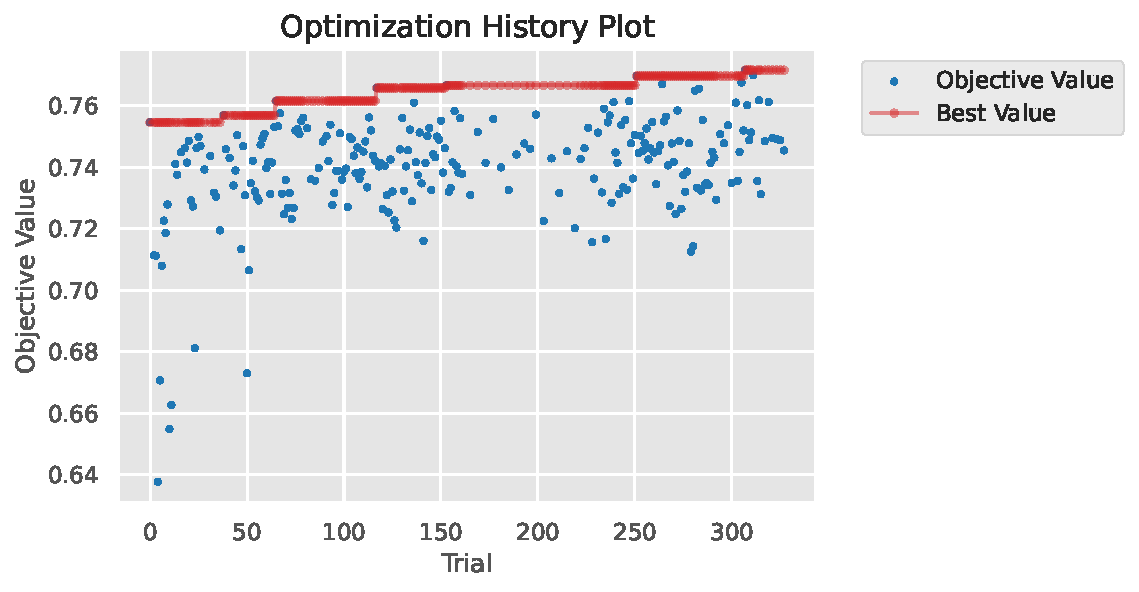
\includegraphics[width=\textwidth]{220915_optimization_history_plot.pdf}
    \caption{Optimization history of the baseline model over a large number of trials, with individual points showing evaluations of $f(x, \theta)$, and points connected by the red line representing the best parameters $\hat{\theta}$ obtained up to that point.}
    \label{fig:hyperparam-optimization-history}
\end{figure}

Early trials result in low objective values because of the essentially random choice of hyperparameters. As the hyperparameter space is explored, the objective value improves logarithmically, though a large variance remains, with little practical performance gains beyond approximately 200 trials. Table \ref{tab:hyperparam-opt-results} documents the values of dataset related hyperparameters as outlined in Section \ref{sec:baseline-hyperparam-tuning}. 


\begin{table}[h]
    \vspace{0.1cm}
    \centering
    \setlength{\tabcolsep}{0.5em}
    \def\arraystretch{1.1}
    \begin{tabular}{L{2.8cm} | L{4cm} | L{2cm} | L{1.3cm} }
    \hline
    Hyperparameter & Description & Range & Best\\
    \hline
    Impute Strategy\textsuperscript{($*$)} & Statistic used to impute missing values & mean, median, most frequent & \textbf{mean}\\
    Grouped Impute\textsuperscript{($*$)} & Impute based on global or per-customer statistics & \emph{T}, \emph{F} & \textbf{\emph{T}}\\
    Drop percentage\textsuperscript{($*$)} & Delete columns with high correlation coefficient & $[0.8; 0.99]$ & $0.94$\\
    Denoise\textsuperscript{($*$)} & Apply denoising strategies & \emph{T}, \emph{F} & \textbf{\emph{T}}\\
    Depth & Tree depth & $\{3; 11\}$ & $11$\\
    Iterations & Number of iterations for regressor & $\{20; 150\}$ & $130$\\
    Learning Rate & Learning rate for regressor & $[10^{-3}; 10^{-1}]$ & $5 * 10^{-2}$\\
    \hline
   \end{tabular}
   \vspace{0.1cm}
   \caption{Best hyperparameters $\hat{\theta}$ after 300 optimization trials achieving a challenge metric of $f(x,\hat{\theta})=0.76$. ($*$) marks dataset parameters reused for deep learning experiments.}
   \label{tab:hyperparam-opt-results}
\end{table}

As a result of the optimization of the \emph{Drop percentage} parameter, ten features were dropped that were highly correlated with other features in the dataset. The fact that the parameter reached the optimal value at $0.94$ and not at an extreme end of the optimization range might indicate that dropping highly correlated features is indeed beneficial for model performance.

That denoising and groupwise imputation strategies might bring a significant performance benefit is further illustrated in the contour plot shown in Figure \ref{fig:hyperparam-dataset-contour-plots--discrete-dataset}, showing the value of $f(x, \theta)$ as pairs of hyperparameters are varied, filling missing values with Gaussian Process Interpolation. Between completely disabling and completely enabling these boolean parameters lies a significant difference of $0.08$ in the final objective value as measured by the final challenge evaluation metric.

% TODO TODO TODO fontsize
\begin{figure}
     \centering
     \begin{subfigure}[b]{0.49\textwidth}
         \centering
         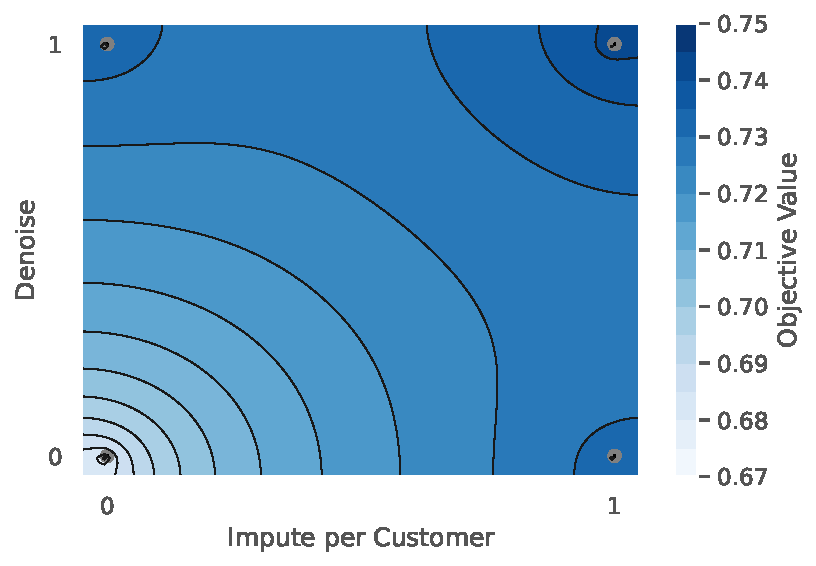
\includegraphics[width=\textwidth]{220915_contour_impute_per_customer_denoise.pdf}
         \caption{Discrete dataset parameters}
         \label{fig:hyperparam-dataset-contour-plots--discrete-dataset}
     \end{subfigure}
     \hfill
     \begin{subfigure}[b]{0.49\textwidth}
         \centering
         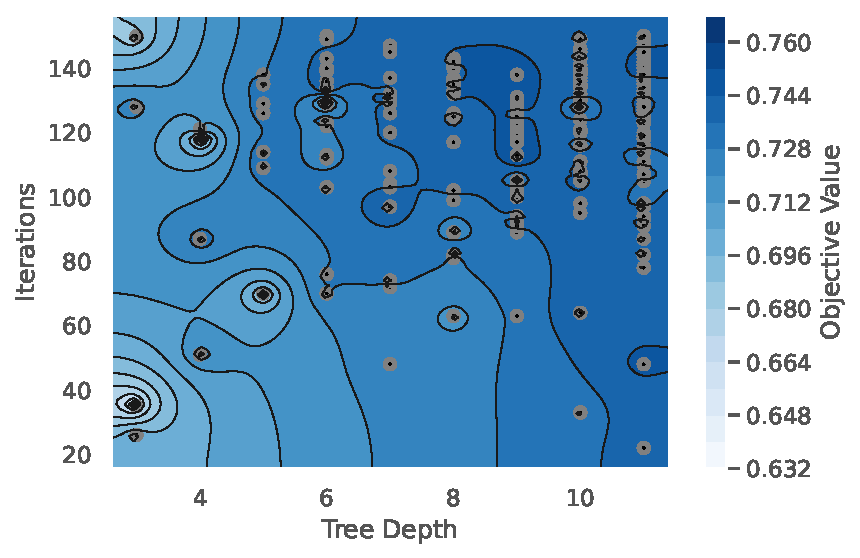
\includegraphics[width=\textwidth]{220915_contour_iterations_vs_tree_depth.pdf}
         \caption{Continuous parameters of GBDT classifier.}
         \label{fig:hyperparam-dataset-contour-plots--continuous-tree}
     \end{subfigure}
    \caption{Contour plots of Gaussian Processes depicting $f$-evaluations as two pairs of hyperparameters are varied (higher objective value is better).}
    \label{fig:hyperparam-dataset-contour-plots}
\end{figure}

Continuous hyperparameters associated with the random forest regressor have a much more complex optimization landscape with many local optima as depicted in Figure \ref{fig:hyperparam-dataset-contour-plots--continuous-tree}, comparing individual tree depth with total number of learning iterations. Despite this, a clear trend towards deeper trees and higher iterations is noticeable, showing that more complicated models tend to be required in order to achieve high evaluation performance. For the tree depth parameter, it is noteworthy this is the only parameter where the boundary of the optimization range has been reached, meaning that possibly tree depth beyond 11 could have further improved the results. However, values beyond 11 could not be explored as the resulting model would exceed the available GPU memory.


% TODO in discussion: this shows that hyperparameter tuning has a significant effect on final performance!
% TODO in discussion: if we don't manage to decrease the variance in later versions of the plot, this means that a lot of non-determinism is in f(x,theta)








\subsection{CNN and MLP Hyperparameter Tuning}
\marginpar{Gann}

In this section, the results of the hyperparameter tuning described in \ref{subsec:hyperparameter-tuning-fcn-cnn} are presented for the MLP and CNN. 

Figure \ref{fig:hyperparam-optimization-fcn-cnn} shows the optimization progress for both MLP and CNN. On the x-axis, the number of trials is shown, while on the y-axis, the objective function is shown, which in this case is the BCE loss. The dots show the loss achieved by a model trained using a selection of hyperparameters. The red line shows the best objective value achieved in the current or earlier trials.


\begin{figure}[h]
     \centering
     \begin{subfigure}[b]{0.49\textwidth}
         \centering
        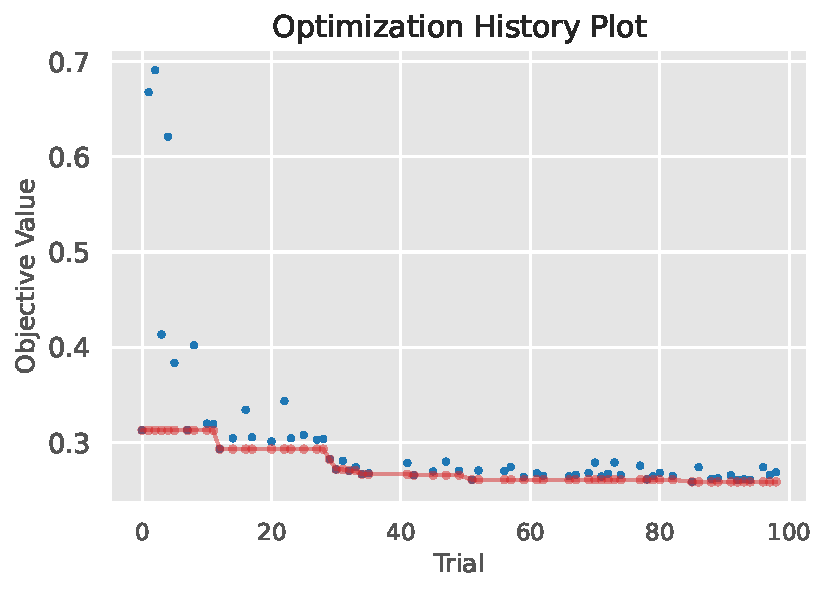
\includegraphics[width=\textwidth]{images/hyper_tuning_lin.pdf}
        \caption{Optimization Progress MLP}

     \end{subfigure}
     \hfill
     \begin{subfigure}[b]{0.49\textwidth}
         \centering
    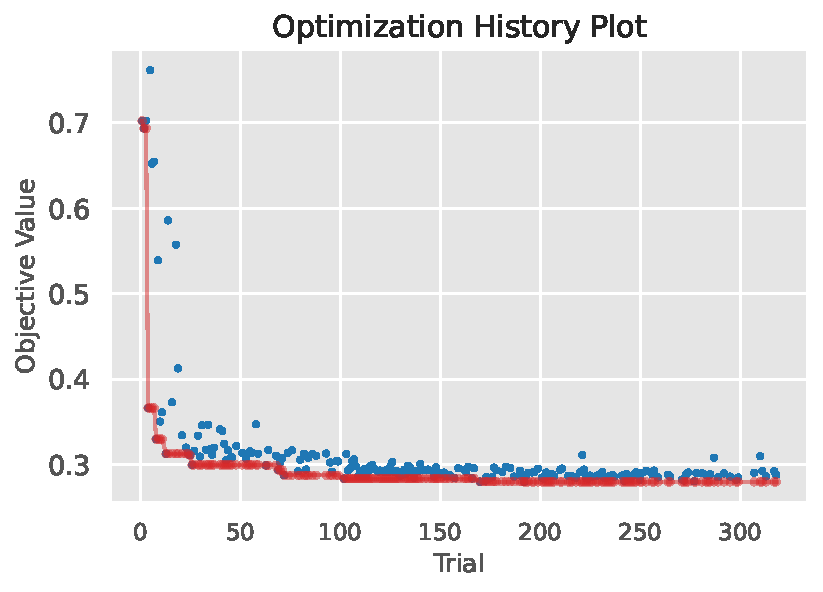
\includegraphics[width=\textwidth]{images/hyper_tuning_conv.pdf}
    \caption{Optimization Progress CNN}

    \end{subfigure}
    \caption{Optimization history plots of deep learning related hyperparameters. The objective value is binary cross entropy (lower is better).}

    \label{fig:hyperparam-optimization-fcn-cnn}
\end{figure}

In both cases, Optuna quickly manages to select hyperparameters, which reduce the loss from about 0.7 to 0.3. It then further optimizes the hyperparameters to gradually achieve a loss of 0.279 in case of the CNN and 0.258 in case of the MLP. For the MLP the optimization was stopped at about 100 trials and in case of the CNN after about 300 trials as no further decrease of the objective value was to be expected.

Using Optuna, the importance of hyperparameters can be quantified. This is done using the fANOVA importance evaluator \cite{pmlr-v32-hutter14}, which fits a random forest regression model that predicts the objective value, allowing for a feature importance analysis through the trained forest in a similar way as described in Section \ref{sec:the-dataset} for dataset feature importances.
Figure \ref{fig:hyperparam-importances-fcn-cnn} shows the importance of the hyperparameters for MLP and CNN.


\begin{figure}[h]
     \centering
     \begin{subfigure}[b]{0.49\textwidth}
         \centering
         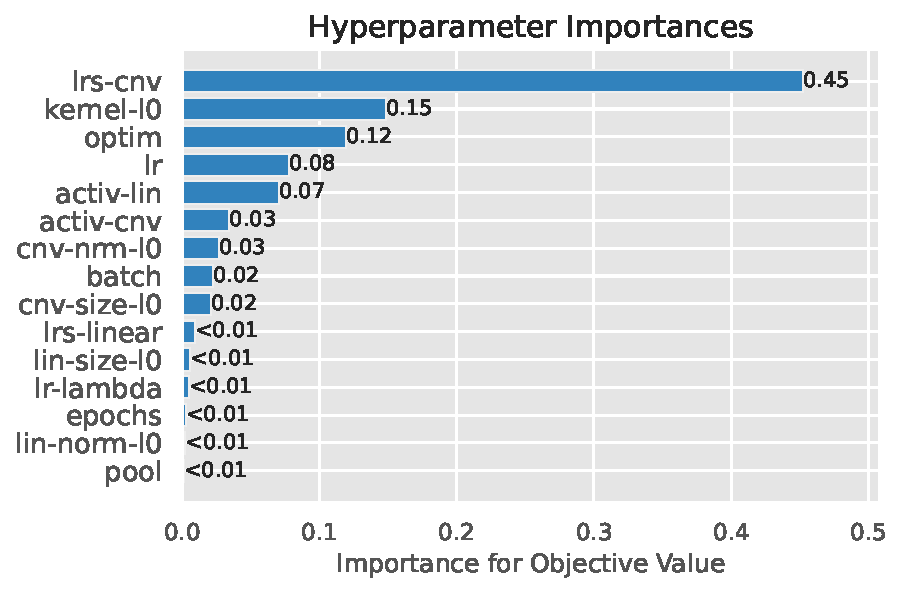
\includegraphics[width=\textwidth]{images/hyper_importances_mlp.pdf}
         \caption{Hyperparameter Importances MLP}
     \end{subfigure}
     \hfill
     \begin{subfigure}[b]{0.49\textwidth}
        \centering
        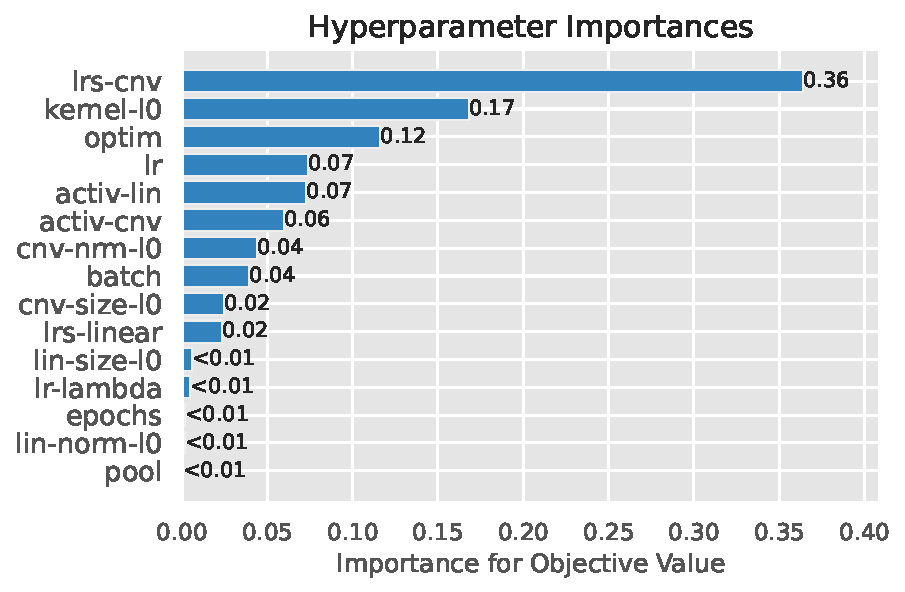
\includegraphics[width=\textwidth]{images/hyper_importances_cnn.pdf}
        \caption{Hyperparameter Importances CNN}
    \end{subfigure}
    \caption{Hyperparameter Importances}
    \label{fig:hyperparam-importances-fcn-cnn}
\end{figure}

The most important hyperparameters in both cases are the total number of initial layers (linear layers in the case of the MLP and convolutional layers in the case of the CNN). The second most important hyperparameter for the MLP is the output size of the first linear layer. For the CNN it is the kernel size of the first convolutional layer. The next two most important hyperparameters in both cases are the optimizer and the learning rate. 

Figure \ref{fig:hyperparam-slice-fcn-cnn} shows the number of layers (linear and convolutional) at which Optuna achieved the best score.

\begin{figure}[h]
     \centering
     \begin{subfigure}[b]{0.49\textwidth}
         \centering
        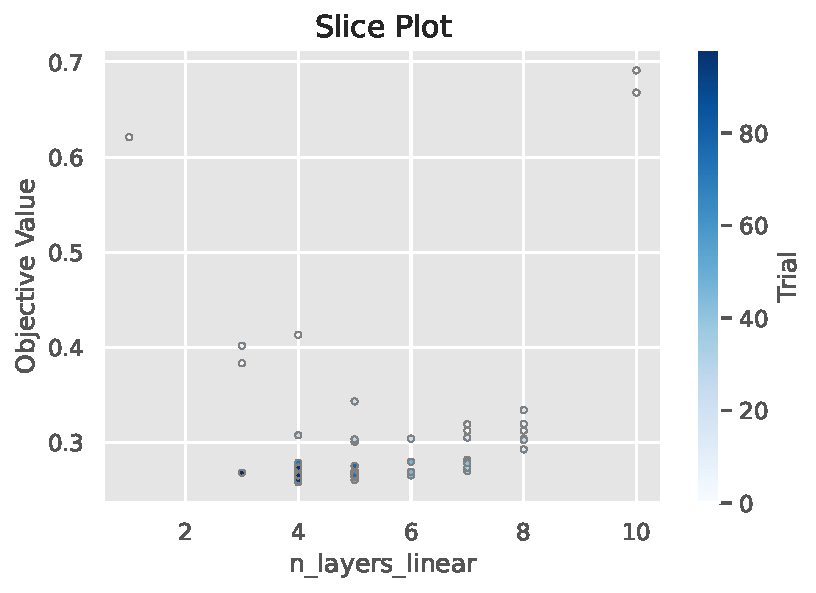
\includegraphics[width=\textwidth]{images/number_layers_mlp.pdf}
        \caption{Slice Plot Linear Layers MLP}

     \end{subfigure}
     \hfill
     \begin{subfigure}[b]{0.49\textwidth}
         \centering
    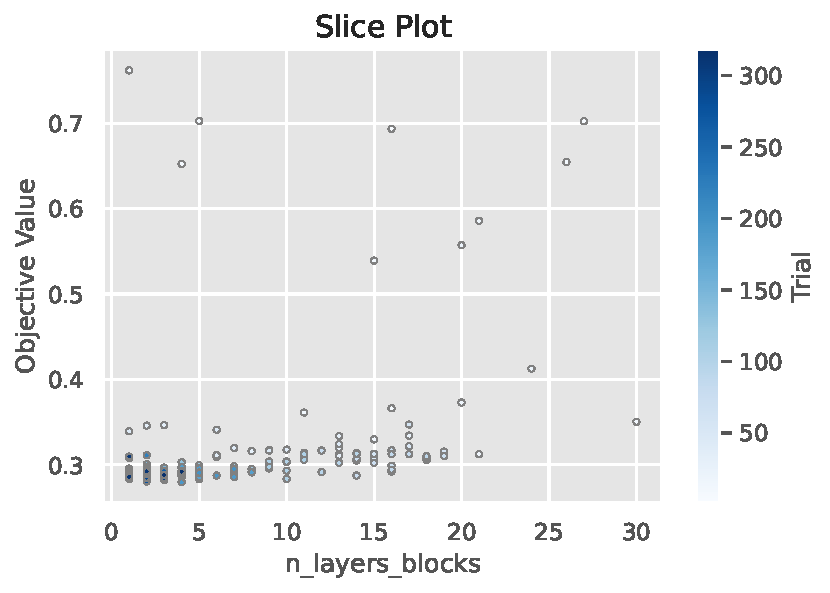
\includegraphics[width=\textwidth]{images/number_layers_cnn.pdf}
    \caption{Slice Plot Convolutional Layers CNN}
    \end{subfigure}
    \caption{Slice Plots Layer Numbers}

    \label{fig:hyperparam-slice-fcn-cnn}
\end{figure}

In both cases, one can see a slight curvature upwards towards the left and right showing a clear optimal value in between.



\subsubsection{Optimized MLP Architecture}

The optimized architecture consists of in total 5 linear layers, the first three layers followed by a ReLU activation, the final layer followed by a Sigmoid function. The output size of the layers are in order: 210, 130, 170, 280, 1. For training, the optimal values were batch size of 80, learning rate of 0.0003, multiplicative learning rate decay of 0.6 and AdamW as optimizer.

% TODO: Plot of model architecture

\subsubsection{Optimized CNN Architecture}

The optimized architecture for the CNN consists of 4 convolutional layers and 7 linear layers. The convolutional layers have in order a kernel size of 9, 12, 5, and 6 and an output size of 300, 200, 180, and 140. Each convolution is followed by a ReLU activation and batch normalization is performed after the activation function on layer 2 and 4.  
The linear layers have in order an output size of 200, 220, 260, 280, 100, 130, 230, 1. Each linear layer is followed by a ReLU activation, but the last activation is a Sigmoid instead of a ReLU. Between convolution and linear layers, a max pool with window size of 13 is performed.

For training, the optimal values were batch size of 112, learning rate of 0.0013, multiplicative learning rate decay of 0.89 and Adam as optimizer.

% TODO: Plot of model architecture



\subsection{Training}
\marginpar{Gann}

Using the training method described in Section \ref{subsec:train-fcn-cnn}, the validation loss of the BCE after every 100 batches is visualized for the MLP and CNN model in Figure \ref{fig:train_loss_fcn-cnn}.


\begin{figure}[h]
     \centering
     \begin{subfigure}[b]{0.49\textwidth}
         \centering
        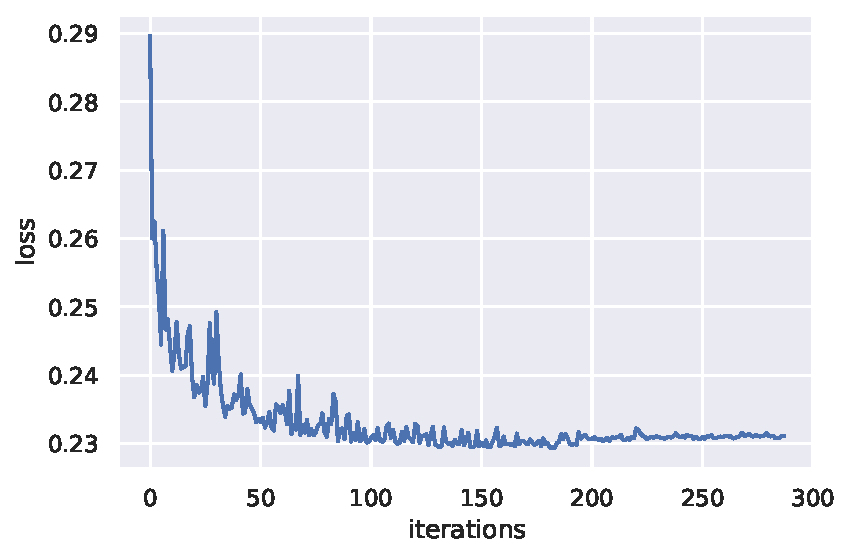
\includegraphics[width=\textwidth]{images/train_loss_lin.pdf}
        \caption{BCE loss for the test set at every 100 batches during MLP training.}

     \end{subfigure}
     \hfill
     \begin{subfigure}[b]{0.49\textwidth}
         \centering
    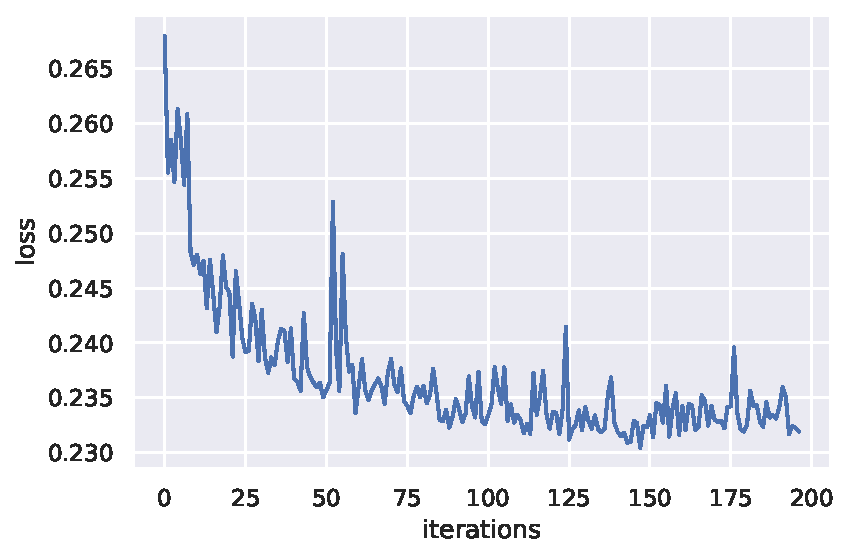
\includegraphics[width=\textwidth]{images/train_loss_conv.pdf}
    \caption{BCE loss for the test set at every 100 batches during CNN training.}

    \end{subfigure}
    \caption{BCE loss curves during training of deep learning approaches.}

    \label{fig:train_loss_fcn-cnn}
\end{figure}

Both curves show a steep decline in the beginning merging into a gradual decline with a slight incline towards the end. One can see that both models reach their optimal classification performance at about 150 iterations, from where on the loss does not decrease but increase. It is also notable that the CNN experiences a greater variance in classification performance throughout the training process. This behavior can be observed up to the end of the training process. Both best performing models of MLP and CNN achieve a BCE loss of 0.23.

The members of the GBDT ensemble as described in Section \ref{sec:gbdt} achieve a mean challenge metric of $0.77$ and minimum BCE loss of $0.25$ as measured on the respective validation folds. On average, peak performance on the validation set is achieved after building around 800 trees, after which the model overfits. For final prediction, trees built after this peak performance has been achieved are removed in order to obtain the state of the best model.

All models were trained on a single Nvidia Tesla V100 GPU with 32GB of available GPU memory using CUDA version 11.4.

\subsection{Validation and Discussion}
\marginpar{Grab, Gann}
\label{sec:experiments-validation}

Figure \ref{fig:dot-plots-individual} visualizes raw per-case assessment data individually for each method, as measured on a reserved testing dataset described in Section \ref{sec:model-evaluation}. While per-case performance is very similar for all methods, overconfident mispredictions resulting in high cross-entropy values are more common for the neural network based approaches. This observation is in line with findings in literature stating that neural networks are more likely to produce overconfident predictions than traditional learning approaches \cite{abdar2021review}.

\begin{figure}
    \centering
    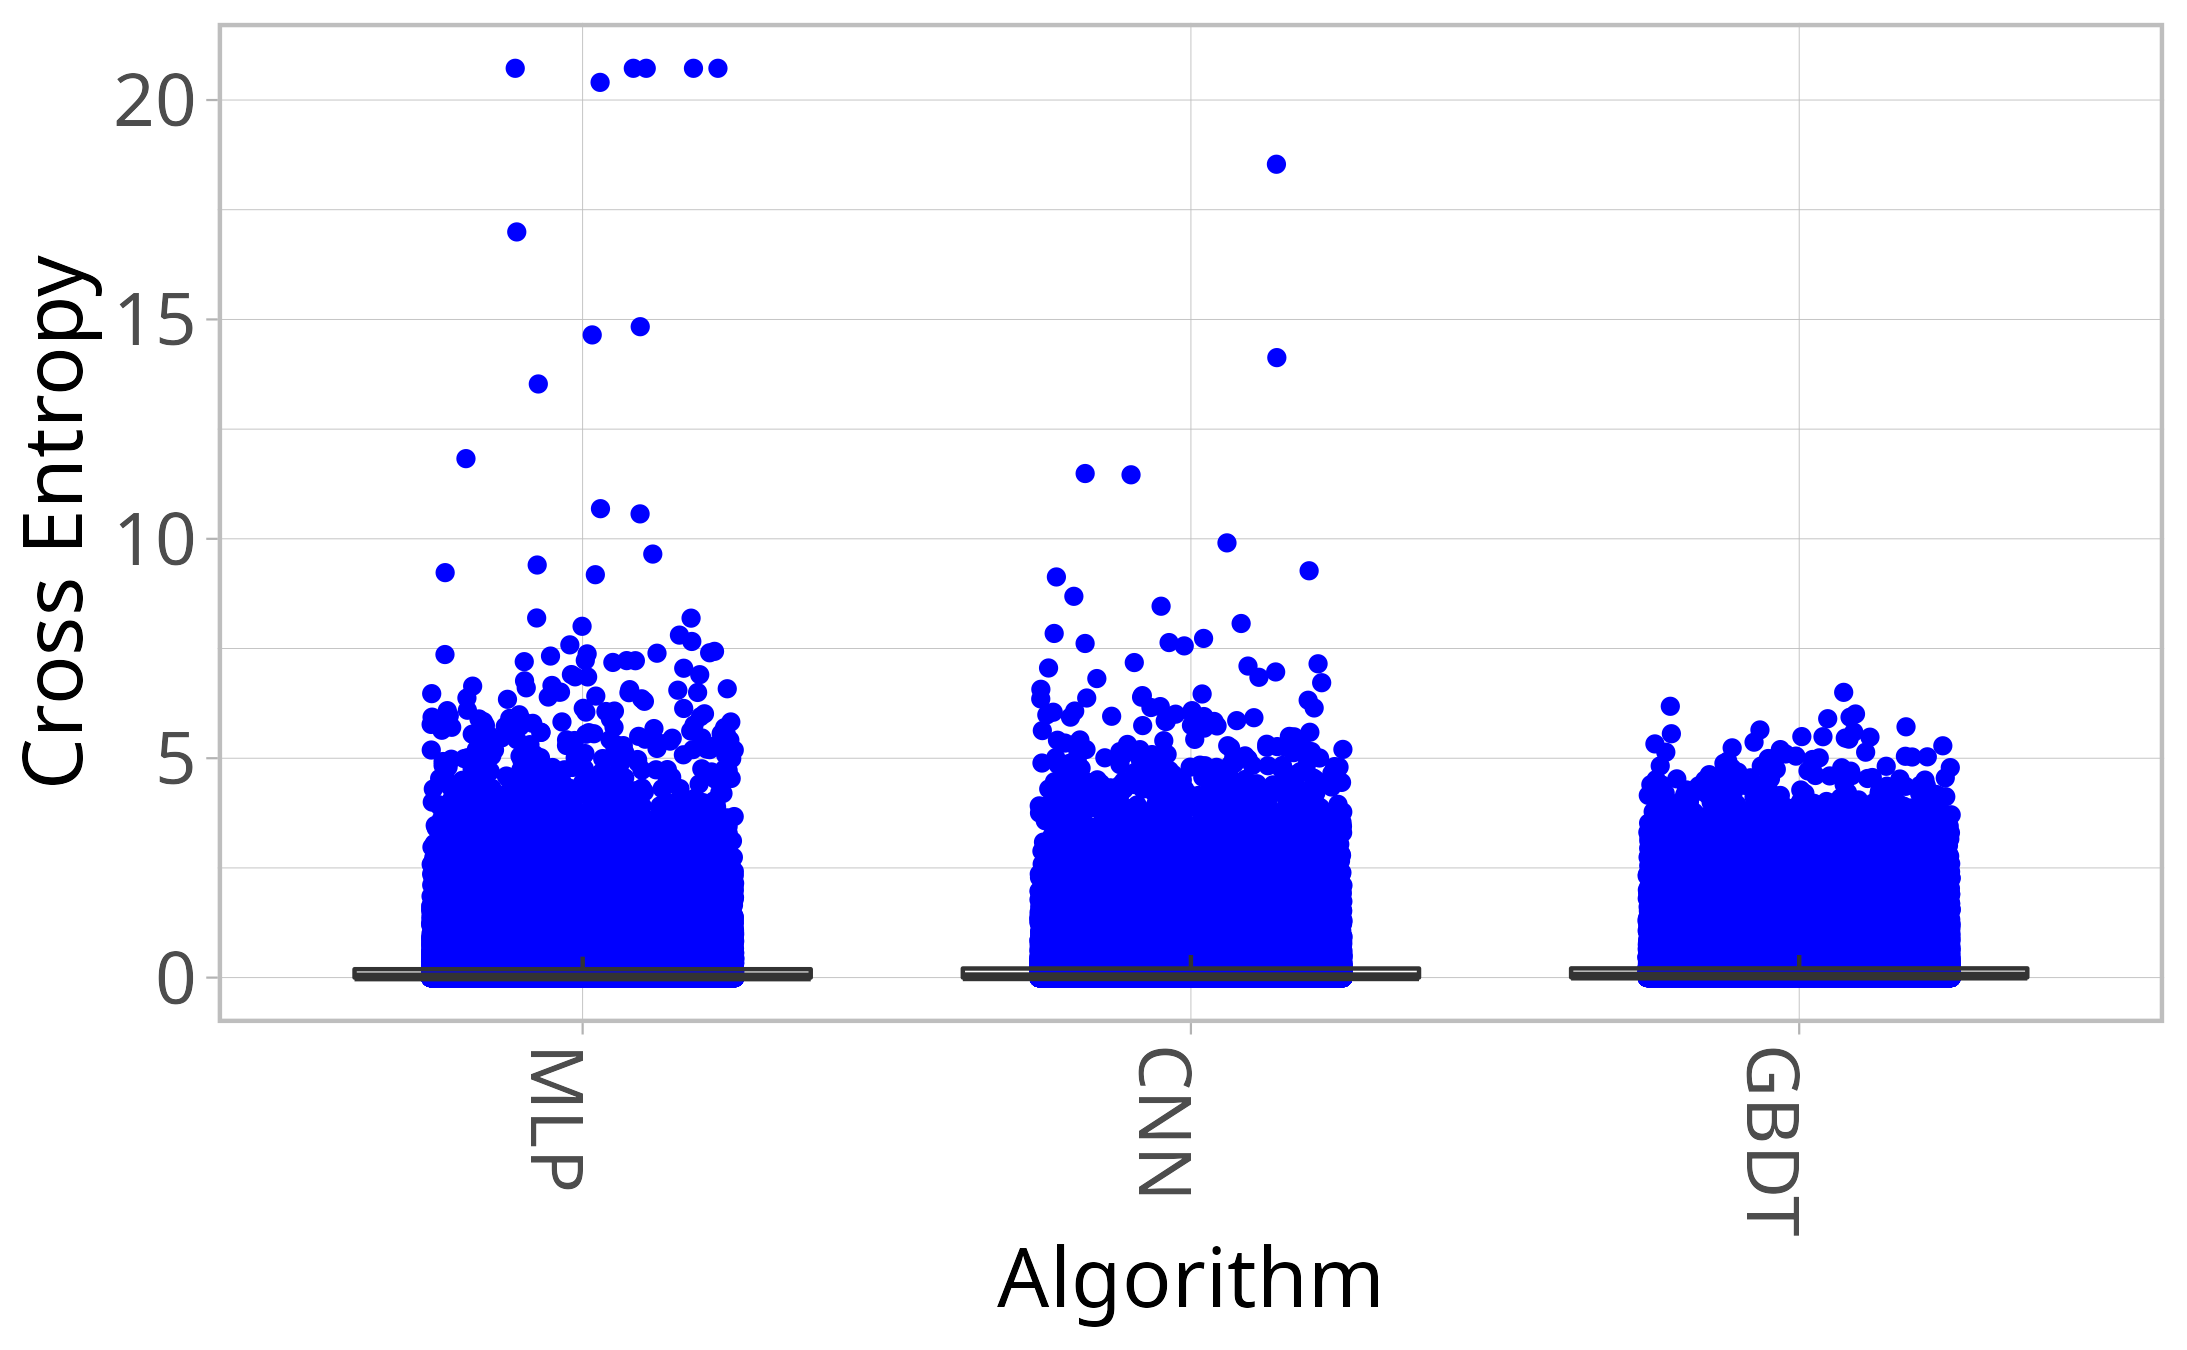
\includegraphics[width=.9\textwidth]{220923_boxplot_ranking_cross_entropy.png}
    \caption{Dot- and boxplots showing individual test-case performance for each method, as determined by binary cross entropy. Lower values are better.}
    \label{fig:dot-plots-individual}
\end{figure}

Table \ref{tab:validation-results} summarizes the final performance metrics achieved with each algorithm, where the first metric column describes the official challenge metric retrieved by submitting predictions to the competition website, and latter metrics were computed on our own test split of the data.
The results show that despite GBDT achieving the highest metric values, all methods lie together closely. Notable in particular is that incorporating time series information in the model as done through the convolutional layers of the CNN had no measurable effect as compared to MLP and GBDT which did not use the time series. One of multiple plausible reasons for this might be that the time series are not long enough for the convolution to leverage its potential in pattern detection. As discussed in Section \ref{subsec:cnn}, the optimal kernel size determined for the first convolution is 9 which indicates that relevant patterns in the input data are about as long as the whole time series. As a result, a convolutional layer with kernel size similar to the channel length has a similar effect as a linear layer. In addition to that, as a result of a kernel size of 9 in the first layer and 12 in the second layer, most of the values in the resulting vectors are padded (for kernel size 12 in layer 2 only 2 values do not result from padding). This greatly diminishes the information on which a convolutional operation can train on. Combined with the observation that for the CNN Optuna optimized to attach 7 linear layers we believe the convolutions did not have a beneficial effect but were optimized to not negatively influence the predictive capabilities of the following MLP. 



\begin{table}[h]
    \vspace{0.1cm}
    \centering
    \setlength{\tabcolsep}{0.5em}
    \def\arraystretch{1.1}
    \begin{tabular}{L{2cm} | L{2.8cm} | L{2.8cm} | L{2cm} }
    \hline
    Method & Kaggle Score & Score (*) & AUC (*)\\
    \hline
    GBDT & \textbf{0.791} & \textbf{0.781} & \textbf{0.959}\\
    MLP & 0.781 & $0.777$ & $0.957$\\
    CNN & 0.783 & $0.776$ & $0.956$\\
    \hline
   \end{tabular}
   \vspace{0.1cm}
   \caption{Final performance metrics of algorithms, with best score of column marked in bold. (*) marks metrics computed on the reserved testing dataset.}
   \label{tab:validation-results}
\end{table}

The Wilcoxon signed rank test described in Section \ref{sec:model-evaluation} as performed on the cross-entropy metric on the reserved testing data revealed that no method was significantly superior to any other method above the significance threshold of 5\%.

The winning submission of the entire challenge achieved a final metric of \emph{0.809}, while our best submission was \emph{0.791}. In terms of leaderboard ranking, comparison is difficult as multiple high scoring ($>0.80$ score) approaches were publicly shared on discussion forums prior to the challenge deadline. Therefore, our best submission is around the center of the global challenge leaderboard.


% TODO zu viel neue information?
Two main differences of the approaches presented in this report and the winning submissions to the challenge can be identified. First, many top performing approaches contain extensive manual feature engineering despite the unique challenge of features being anonymized. This includes deriving new kinds of features by means of aggregating the time series in certain ways, whereas we rely on the Neural Network and GBDT architectures to implicitly derive useful combined features. Second, most winning approaches use weighted ensembles of different network architectures in a technique called stacking to take advantage of the fact that different machine learning approaches learn differently from the same data, and thus combine the advantage of multiple methodologies. 


%Results on test set:
%Accuracy: 89.7\%
%Avg loss: 0.238998 
%precision: 0.8968

%recall: 0.8968

%amex-score: 0.7706765075408728


%f1 tensor(0.8968, device='cuda:0')

%\begin{enumerate}
%    \item list scores of validation set (accuracy, loss, amex-metric)
%    \item list scores of amex metric for submitted test set 
%\end{enumerate}


% Preprocessing & Hyperparameter
% Data Exploration: Feature importance, Imputation, etc
% Embeddings
% Baseline Random Forest
% Resnet
% CNN
% LSTM
% Graph mit Loss functions, etc
% Kaggle Metrik, Epoche für Epoche oder einmal am Ende

% Vergleich DL Modelle/normale mit normalem Preprocessing & Embeddings


% Conclusion
% -> 


%Having introduced our methods, we now give quantitative insights into their performance of learning to classify risk of credit default. 

% \emph{TODO welche experimente..}

%\subsection{Baseline Random Forest}
% Notebook: 220819_explore_naive_catboost.ipynb
%As Random Forest based models have a good track record of working on tabular data, the first experiments were based on them in order to create a performance baseline. The data was only preprocessed minimally. Categorical features were transformed to suitable one-hot-encoded representations and string columns such as the statement date were removed entirely. CatBoost was used as the implementation of gradient boosted trees due to its ability to handle categorical features with little effort \cite{dorogush2018catboost}. Training was done row-wise, meaning that the temporal information of a customer was discarded entirely. The target label was set to the customer outcome (default or no default) for each row and training was conducted over 1000 iterations. Prediction on the test dataset was again conducted row-wise, and predicted probabilities were averaged over all customer records with equal weights to obtain the final predicted probability of the default event. This approach achieved a score of \emph{0.71} as measured on the test dataset.

%\subsection{Wide Random Forest}
% Notebook: 220820_catboost_combined_rows.ipynb
%Already 0.72 score only trained on 5000 customers, seems promising
%every record belonging to customer goes on one line
% Score of 0.77 on full network and finetuned with cross-val/grid search
% Notebook: 220822_catboost_combined_rows_finetune_pred.ipynb

% Tabnet (DNN): Nur ca. 0.76, schlechter als trees.

\section{Conclusion}
\label{sec:conclusion}
\marginpar{Grab, Gann}

% Public availability of test set was criticised by some - self supervised training of for example embeddings was possible.
% TODO citations in conclusion ok?? can't remember...

In this report, we investigated the problem of predicting whether credit card customers default on their loans given past performance indicators using a large, industry scale dataset provided by the lending institution American Express.
In particular, we explored whether deep learning approaches could be successfully applied to the problem, whereby we mean whether deep learning approaches are able to surpass approaches known to work well on similar data such as GBDT. To answer this question, we trained GBDT, MLP, and CNN models using identical basic data preprocessing procedures. In both preprocessing and training, we heavily relied on automated hyperparameter optimization based on Gaussian Processes to systematically determine good parameters. Our results replicate prior work in the area indicating deep learning models approach similar performance, but fail to surpass GBDT in predictive accuracy \cite{alam2020investigation}. In particular, we show that Neural Network approaches are more susceptible to overconfident misclassifications, again confirming prior work \cite{abdar2021review}.


\subsection{Limitations}
\marginpar{Grab, Gann}


In order to allow for fair comparison between the deep learning methods and GBDT, we used hyperparameter optimization in our preprocessing pipeline that itself uses GBDT for evaluation purposes. While the results of hyperparameter optimization are qualitatively sensible, they might thus be biased towards GBDT, giving the deep learning methods a disadvantage. However, as evaluating performance using deep learning approaches would have been too expensive computationally, the only alternative we see is manually specifying the data preprocessing pipeline, which also could be implicitly biased towards one specific method. A different consideration regarding the optimization is that the objective functions are non-deterministic in all cases and thus have some amount of variance attached, which we did not consider further in this report.

In this report, we only present two deep learning architectures. While it should be noted that the CNN architecture is mostly used for Computer Vision problems, we conjectured that the concept of convolutions might also bring a beneficial effect in the context of time series data, though we could not confirm this experimentally. In early experiments, different architectures such as Long Short-Term Memory (LSTM) and Recurrent Neural Networks were used, but results obtained were broadly similar to CNN and MLP and thus these experiments were not included in this discussion.

%We, however, found indications that, due to the small length of the time series, convolutions had a detrimental effect on classification performance and were made ineffective during hyperparameter optimization, essentially reducing the CNN to an MLP.





\subsection{Future Work}
\marginpar{Grab, Gann}

Credit default prediction remains an interesting avenue for machine learning; however, it is important not to completely leave practical application out of sight. Considering a potential use case where, for example, high default risk customers are identified as early as possible and their contracts terminated, regulatory compliance and, more precisely, explainability should be a focus of future machine learning experiments. While GBDT are more explainable models than most, an interesting consideration could be whether alternative approaches with explanatory components such as Invertible Neural Networks could be used successfully in this context.

Returning to a more theoretical consideration, given the success of ensemble approaches stacking different kinds of machine learning methodologies, an interesting question is whether combining the approaches presented in this report in certain ways would lead to better predictive performance than the approaches individually.

Finally, in a broader picture than the specific problem of credit default prediction, it remains interesting to see that in learning from structured, tabular data, deep learning still does not live up to its high expectations set by unprecedented successes with processing unstructured, large-scale, or noisy data such as in computer vision or audio recognition. Determining why precisely this is the case and exploring alternative deep learning methodologies with increased potential to exploit tabular structures remains an exciting open area of research.

%TODO FUTURE WORK: Stacking has won the competition. We didn't use stacking. Use stacking the future.
%TODO for DL based hyperparameter tuning, potentially cite the variance in DL paper.
%imply good performance with deep learning approaches. - However, the parameters found by the optim were found to be sensible, also DL based hyperparam optim might have been too costly
%TODO vielleicht etwas auf bezug zu explainable AI: \cite{Rudin2019Why}
%Their score is an overall performance metric (AUC etc). Doesnt say much, how about sensitivity/specificity?

%\begin{enumerate}
%    \item effects of low confidence postive classification => other possible metrics?
%    \item why MLP and CNN equally good? possibly because time series not long enough: first layer %kernel size of cnn is 9 which is most of the time points => relevant patterns in input data have %almost the same size as the whole input
%    \item observation: CNN "requires" many linear layers (7)
%\end{enumerate}

\clearpage
\appendix
\bibliographystyle{splncs04}
\bibliography{bibliography}
%
\end{document}
